\documentclass[12pt,]{article}
\usepackage[left=1in,top=1in,right=1in,bottom=1in]{geometry}
\newcommand*{\authorfont}{\fontfamily{phv}\selectfont}
\usepackage[]{mathpazo}


  \usepackage[T1]{fontenc}
  \usepackage[utf8]{inputenc}




\usepackage{abstract}
\renewcommand{\abstractname}{}    % clear the title
\renewcommand{\absnamepos}{empty} % originally center

\renewenvironment{abstract}
 {{%
    \setlength{\leftmargin}{0mm}
    \setlength{\rightmargin}{\leftmargin}%
  }%
  \relax}
 {\endlist}

\makeatletter
\def\@maketitle{%
  \newpage
%  \null
%  \vskip 2em%
%  \begin{center}%
  \let \footnote \thanks
    {\fontsize{18}{20}\selectfont\raggedright  \setlength{\parindent}{0pt} \@title \par}%
}
%\fi
\makeatother




\setcounter{secnumdepth}{0}

\usepackage{longtable,booktabs}



\title{(Work in Progress) Political Donor Polarization: Observing Consumptive
Behavior using a Network Approach  }



\author{\Large \vspace{0.05in} \newline\normalsize\emph{}  }


\date{}

\usepackage{titlesec}

\titleformat*{\section}{\normalsize\bfseries}
\titleformat*{\subsection}{\normalsize\itshape}
\titleformat*{\subsubsection}{\normalsize\itshape}
\titleformat*{\paragraph}{\normalsize\itshape}
\titleformat*{\subparagraph}{\normalsize\itshape}





\newtheorem{hypothesis}{Hypothesis}
\usepackage{setspace}


% set default figure placement to htbp
\makeatletter
\def\fps@figure{htbp}
\makeatother

\usepackage{graphicx}

% move the hyperref stuff down here, after header-includes, to allow for - \usepackage{hyperref}

\makeatletter
\@ifpackageloaded{hyperref}{}{%
\ifxetex
  \PassOptionsToPackage{hyphens}{url}\usepackage[setpagesize=false, % page size defined by xetex
              unicode=false, % unicode breaks when used with xetex
              xetex]{hyperref}
\else
  \PassOptionsToPackage{hyphens}{url}\usepackage[draft,unicode=true]{hyperref}
\fi
}

\@ifpackageloaded{color}{
    \PassOptionsToPackage{usenames,dvipsnames}{color}
}{%
    \usepackage[usenames,dvipsnames]{color}
}
\makeatother
\hypersetup{breaklinks=true,
            bookmarks=true,
            pdfauthor={ ()},
             pdfkeywords = {polarization, political donations, network analysis, state politics},  
            pdftitle={(Work in Progress) Political Donor Polarization: Observing Consumptive
Behavior using a Network Approach},
            colorlinks=true,
            citecolor=blue,
            urlcolor=blue,
            linkcolor=magenta,
            pdfborder={0 0 0}}
\urlstyle{same}  % don't use monospace font for urls

% Add an option for endnotes. -----


% add tightlist ----------
\providecommand{\tightlist}{%
\setlength{\itemsep}{0pt}\setlength{\parskip}{0pt}}

% add some other packages ----------

% \usepackage{multicol}
% This should regulate where figures float
% See: https://tex.stackexchange.com/questions/2275/keeping-tables-figures-close-to-where-they-are-mentioned
\usepackage[section]{placeins}


\begin{document}
	
% \pagenumbering{arabic}% resets `page` counter to 1 
%
% \maketitle

{% \usefont{T1}{pnc}{m}{n}
\setlength{\parindent}{0pt}
\thispagestyle{plain}
{\fontsize{18}{20}\selectfont\raggedright 
\maketitle  % title \par  

}

{
   \vskip 13.5pt\relax \normalsize\fontsize{11}{12} 
\textbf{\authorfont } \hskip 15pt \emph{\small }   

}

}








\begin{abstract}

    \hbox{\vrule height .2pt width 39.14pc}

    \vskip 8.5pt % \small 

\noindent American politics has recently been defined by unprecedented levels of
partisan polarization. Given the concurrent rise of the amount of money
in politics, many have suggested a connection between money in politics
and polarization. This paper uses the occurrence of a specific
polarizing event, former Wisconsin Governor Scott Walker's introduction
and passage of Act 10, to analyze the relationship between donor
polarization and mass polarization. Using political donation data from
the Wisconsin Campaign Finance Information System (CFIS) and using the
network science measure of modularity, this paper shows that political
donor networks polarized during the 2012 election cycle at the same time
as the electorate. This result suggests that political donors were
likely not the main contributors to the polarization in the state and
provides evidence for the `consumption' model of political donations.


\vskip 8.5pt \noindent \emph{Keywords}: polarization, political donations, network analysis, state politics \par

    \hbox{\vrule height .2pt width 39.14pc}



\end{abstract}


\vskip -8.5pt


 % removetitleabstract

\noindent \doublespacing 

Political campaign finance plays an important role in the American
political system. This significance is evidenced by the attention that
academic researchers pay to the topic as well as the many different
contexts in which campaign finance is studied. For example, research has
concluded that: campaign contributions ultimately impact one-third of
all congressional roll-call votes (Roscoe and Jenkins 2005), even small
contributions can sway politicians' votes (Stratmann 1991), campaign
finance is a contributor to gender inequities between the Democratic and
Republican parties (Barber, Butler, and Preece 2016; Crowder-Meyer and
Cooperman 2018; Kitchens and Swers 2016; Thomsen and Swers 2017),
existing professional networks are beneficial to new politicians (Bonica
2017), and candidates spend a significant amount of time fundraising
(Torres-Spelliscy 2017). In addition, the concurrent rise of money in
politics and political polarization has led to the idea that the two are
connected (Francia et al. 2005; McCarty, Poole, and Rosenthal 2006).
Barber (2016) concludes that ``the connection between donors and
candidates is an important part of the story of the polarization of
American politics''.

The folk-theory of political donors is of smokey backrooms and
access-oriented donors who seek to have a direct influence on policy
making. However, the psychological processes of donors are thought to be
similar to ordinary voters. Political donations can be thought of an
extension of voting. In other words, both actions are political
consumption that seek to improve a preferred candidate's chances of
winning. Ansolabehere, de Figueiredo and Snyder summarized this idea by
stating, ``In our view, campaign contributing should not be viewed as an
investment, but rather as a form of consumption---or, in the language of
politics, participation'' (Ansolabehere, Figueiredo, and Jr. 2003).

Donations can be seen as an outlet for motivated citizens to increase
their participation beyond just turning out to vote when they perceive
the stakes of elections to be high (Hill and Huber 2017). Even when
individuals have an economic interest in the outcome of an election,
donations are found to be motivated by existing policy agreements and
not an expectation of access (Barber, Canes-Wrone, and Thrower 2016).
For example, donations from business executives have been found to be
``best understood as purchases of `good will' whose returns, while
positive in expectation, are contingent and rare'' (Gordon, Hafer, and
Landa 2007).

Although the psychological process of making a political campaign
contribution can be thought of as similar to voting, there are
significant demographic and ideological differences between donors and
voters. People with lower incomes, less education, and those not in
professional jobs are less likely to be politically engaged, including
making political donations (Laurison 2016). Donors to the Democratic and
Republican parties were previously summarized as being ``Limousine
Liberals'' and ``Corporate Conservatives'' (Francia et al. 2005).
However, that narrative has shifted recently in the wake of the
\emph{Citizens United} supreme court case which allowed individuals to
contribute more money to political causes and the rise of small-dollar
donors (Albert and Raja 2020).

While Democrats and Republicans draw their bases of electoral support
from different geographic bases, major campaign donors are highly
concentrated geographically. These ``big-donor neighborhoods'' are
unrepresentative of the country as a whole and point to these
communities having a distinct political culture (Bramlett, Gimpel, and
Lee 2011). In both parties, donors are more ideologically extreme than
non-donating voters (Francia et al. 2003; Hill and Huber 2017) and
wealthy donors who make up the ``big money'' in politics are especially
partisan (McCarty, Poole, and Rosenthal 2006).

This ideological extremity shown by political donors has led some
scholars to suggest that political donors are contributors to the
partisan polarization of the politics of the United States (Francia et
al. 2005). This idea is supported by the observation that both political
polarization and campaign spending have risen in conjunction (McCarty,
Poole, and Rosenthal 2006). Despite this observed correlation, there is
little evidence for the causal relationship of donors causing political
polarization. Many have found that political donations don't influence
polarization (Harden and Kirkland 2016; Keena and Knight-Finley 2019;
Raja and Wiltse 2012). Furthermore, it is likely the case that the
causal arrow flows the other direction, and it is a more polarized
electorate and candidates that have led to more polarized donors (Harden
and Kirkland 2016; Keena and Knight-Finley 2019; Raja and Wiltse 2012).

If political donors were found to be contributors of political
polarization, the ever-growing amount of money in politics could
forewarn even greater levels of polarization. In addition, political
donors contributing to polarization would mean that donors are even more
influential in the broader realm of politics than previously believed.
Further, there could be policy responses to attempt to curb the amount
of money in politics and therefore political polarization, such as more
strict contributions limits.

Studying polarization, particularly among political donors can be
difficult because of the myriad of potential confounding factors that
can contribute to polarization (Harden and Kirkland 2016). In addition,
polarization is generally a phenomenon that gradually increases or
decreases over time (Pew Research Center 2017). However, this paper
leverages a singular event, former Wisconsin Governor Scott Walker's
proposition and passage of Act 10, a ``budget repair bill'' that ended
collective bargaining for teachers unions, to examine political donor
polarization in the state of Wisconsin. Given the recent research which
has pointed to the polarization of political donors as being
\emph{reactive} instead of \emph{causal} to broader polarization, we
could expect political donors to follow the trend of voters and polarize
after introduction of Act 10 and subsequent events. Particularly, we
would expect levels of polarization among political donors to be closely
aligned with levels of polarization of the mass electorate under the
consumption model of political donations where donations are a
participatory extension of voting.

\textbf{\(H_{1}\): Political donors in the State of Wisconsin polarized
during the 2012 election cycle compared to the 2010 election cycle and
maintained their level of polarization in the 2014 election cycle.}

If this hypothesis is supported, these results would strengthen the
evidence for politics donors being \emph{reactive} to their political
environment as we would expect under Ansolabehere, de Figueiredo and
Snyder's consumption model of political giving.

Alternatively, if political donors are instead \emph{contributors} to
mass and legislative polarization, as is suggested by some scholars, we
would expect to see hypothesis two.

\textbf{\(H_{2}\): Polarization levels stayed the same in the 2012
election cycle compared to the 2010 election cycle.}

If hypothesis two is supported, the result would suggest that political
donors helped to create the polarized political environment that we see
today.

In addition, this paper makes a methodological contribution to campaign
finance research by taking a network approach to measuring donor
polarization by using modularity as a measure of polarization. This
method has been used elsewhere in the social sciences to study
congressional polarization (Waugh et al., n.d.; Zhang et al. 2008) and
polarization in social media networks (Conover et al. 2011; Garcia et
al. 2015; Guerra et al. 2013). This paper conceives of the political
donor landscape of donors and candidates acting as nodes who are
connected by donations that act as edges. This method is important in
studying political donor networks because it takes into consideration
real-world actions, such as in network studies of polarization among
member of congress where voting records (Guerra et al. 2013) and
co-sponsorships (Zhang et al. 2008) are used to study polarization
opposed to surveys administered to donors that rely on self-reported
ideology and partisanship.

\hypertarget{wisconsin-context}{%
\section{Wisconsin Context}\label{wisconsin-context}}

Both Wisconsin's legislators and mass public are among the most
polarized in the nation (Cramer 2016), and the state has been used by
academics to examine how political actions unfold in contentious and
highly divisive environment (Bode et al. 2018). Although many state
legislatures are also experiencing polarization (Shor 2015), Wisconsin
is unique in that there is a single event that many point to in creating
``the most politically divisive place in America'' (Kaufman 2012).

In 2011, newly-elected Republican Governor Scott Walker introduced Act
10, a ``budget reconciliation bill'' that stripped public school
teachers of collective bargaining via their union. Up to 100,000 people
protested this ``anti-union bill'' at the State Capitol and even
occupied the capitol building for a period of time (Sewell 2011).
Democratic lawmakers fled to Illinois in an effort to delay or stop the
bill from passing into law (Layton 2011). In 2012 there was an
unsuccessful election to recall Governor Walker.

Wisconsin Governor Scott Walker's self-anointed ``divide and conquer''
politics (Blake 2012) has left a political divide in Wisconsin that
persists to today. The result is that ``divisive politics ruled
Wisconsin over the last decade'' (Marley and Beck 2019). The Marquette
Law School poll headed by Charles Franklin has called public opinion in
Wisconsin a ``lesson in the two worlds of Wisconsin'' where ``it seems
often as if people have not only differing opinions but differing views
of facts and realities'' (Borsuk 2017). This discrete event and its
long-lasting consequences provides a unique opportunity to study
massively polarized politics that can be attributed back to a single
event. In addition, Wisconsin is a competitive swing state that reflects
a roughly 50-50 split similar to the country as a whole.

\hypertarget{methodology}{%
\section{Methodology}\label{methodology}}

All data on political contributions came from the Wisconsin Campaign
Finance Information System (``Wisconsin Campaign Information System,''
n.d.). I exported all contributions to State Assembly, State Senate, and
Gubernatorial races from the 2010, 2012, and 2014 elections. This
dataset does not include donations to party committees, although it does
include disbursements from these committees. I manually created a table
of the parties of each of all the campaigns receiving contributions in
this timeframe and added the party of the campaign receiving the
donation to this dataset.

To clean and analyze my data I used the statistical programming language
R (R Core Team 2013; Wickham et al. 2019). I started with 1,499,603
donations. I then filtered out 3,503 unitemized/ anonymous donations,
removed punctuation from the names of the donors, and used Open Refine
(Kelli 2013) via the \texttt{refinr} R package (Muir 2018) to
standardize names (for example, Jim versus James). Next, I created a
unique identifier for donors by combining their standardized name with
their zip code. This identifier was created to be able to link donors
who contributed across multiple campaigns in multiple years without
considering two different people, with the same name, from different
locations to be the same person. Identity resolution is notoriously
difficult and is the biggest limitation of this paper. This study uses
some of the most advanced identity resolution techniques available, but
there is always inevitable error. While this potential error is
difficult to calculate, we expect that any error would be random
distributed across the three election cycles. In other words, one can
assume that the levels of error are the same across all three election
cycles. So, the directional conclusions of this paper remain valid.

Next, I estimated the partisanship of each donor in each election cycle
by taking the percent of donations that each donor gave to Republicans
divided by their donations to Republicans and Democrats. I took that
``percent donated to Republicans'' and rescaled it from -1 to 1, where
-1 represents the most Democratic donors, and 1 the most Republican
donors. I also calculated each individual's party bin: if more than 75\%
of donations were to Democrats, they were labeled as a Democrat; if more
than 75\% of donations were to Republicans, they were labeled as a
Republican; if their donations were somewhere inbetween, they were
labeled as being a bipartisan donor.

To quantify the levels of polarization in each election cycle, I
calculated two statistics: network modularity and average absolute
partisanship of donors.

First, political donations can be thought of as a network where donors
and candidates are nodes and donations connecting donors and candidates
are edges. This conceptualization of the political donor landscape as
network allows us to examine the network structure and calculate network
statistics on the graph of donors and candidates. One of the most useful
network statistics for measuring polarization in a network is modularity
(Newman 2006).

The modularity of a graph measures the strength of the division of
groups (such as political parties) by calculating ``the number of edges
falling within groups minus the expected number in an equivalent network
with edges placed at random'' (Newman 2006). The modularity of a network
falls in the range {[}-1/2, 1{]}. If the modularity is positive, the
number of edges that remain within each group is greater than the
expected number to remain in-group based on chance. The higher the
modularity, the greater the concentration of edges within each groups.
In other words, the higher the modularity of a network, the higher the
polarization among the groups. Formally, the equation to calculate
modularity Q is:

\[Q = \frac{1}{2m} \sum_{ij}\left[A_{ij} - \frac{k_{i}k_{j}}{2m} \right]\delta(g_{i},g_{j})\]

In this equation \(m = \frac{1}{2}\sum_{i}k_{i}\) is equal to the
strength of all the ties in the network, \(k_{i}=\sum_{j}A_{ij}\) is the
strength/ weighted degree of the \(i\)th node, \(g_{i}\) is the group
(in this case, party/ party bin) to which the \(i\) belong, and
\(\delta(g_{i},g_{j}) = 1\) if \(i\) and \(j\) belong to the same group
(party/ party bin) and 0 if they do not belong to the same party/ party
bin.

I calculated the modularity of the network graphs of each election cycle
(2010, 2012, 2014) using the \texttt{igraph} R package (Csardi and
Nepusz 2006). I used candidates' declared parties and donors' party bin
as the groups for the modularity calculation. The modularity of the
network graph of each election is in Table 1.

In addition to calculating the change in modularity of each of the
election cycles, I also analyzed the change in mean absolute
partisanship of the donors in each election cycle (see Table 2).

I defined a donor's absolute partisanship as the absolute value of their
partisanship score (which is on a scale from -1 to 1). Therefore, the
larger a donor's absolute the partisanship, the higher percentage of
their money that they contributed to a single party. To calculate the
significance in the difference of the mean absolute partisanship, I use
a bootstrap methodology with 1,000 replications using the \texttt{infer}
R package (Bray et al. 2020). This paper uses a non-parametric
permutation method because of the non-Normal distribution of
partisanship of the donors (98\% of donors across all election cycles
only contribute to a single party).

These measures of polarization among Wisconsin donors can be compared to
party identification among likely voters in Wisconsin in Table 3 for
2010 (Kniss 2010), 2012, and 2014 (Franklin, n.d.).

\hypertarget{results}{%
\section{Results}\label{results}}

The results of this analysis show that political donors in Wisconsin
polarized during the 2012 election cycle, the same time that mass
polarization occurred in the state (see Table 3). This phenomenon is
best visualized in Figure 1. This figure uses the Yifan Hu layout
algorithm (Hu 2005) in the Gephi software (Bastian, Heymann, and Jacomy
2009), a force-directed graphical layout of networks that seeks to
repulse clusters of nodes from one another. The Yifan Hu layout
algorithm is a standard among social scientists studying networks such
as online networks (Adalat, Niazi, and Vasilakos 2018; Hemsley et al.
2015; Khonsari et al. 2010; Rehman et al. 2020). This visual
representation shows two distinct clusters of donors (Democrats and
Republicans) that are reasonably close to one another in the 2010
election cycle and then polarize significantly in the 2012 election
cycle and remain polarized in 2014.

This graphical representation reflects statistical measures of
polarization within the networks. Table 1 shows the modularity of the
networks in the 2010, 2012, and 2014 election cycles. In 2010, the
modularity of the donor network is 0.4. The modularity for the 2012
cycle climbs to 0.49 and settles in at 0.48 during the 2014 cycle. The
interpretation of modularity is the higher the number, the more observed
polarization within the network. As such, the rise in modularity in the
2012 cycle depicts polarization within the donor network in 2012
compared to 2010. And then the steady modularity in the 2014 cycle
reveals a stabilization of the level of polarization observed in the
2012 election cycle.

One limitation of a modularity calculation is that it does not quantify
uncertainty. To validate the results of the modularity calculation, I
conducted a hypothesis test. Table 2 compares the average absolute donor
partisanship in 2012 compared to 2010 and 2014 compared to 2012. As the
table shows, donors in the 2012 election cycle became much more partisan
with an average change in their absolute partisanship of 0.04211 (CI =
0.04022-0.04395, p-value = \textless.001). However, there was not a
statistically signiciant change in mean absolute partisanship in the
2014 election cycle compared to the 2012 election cycle
(\ensuremath{-2.9\times 10^{-4}}, CI = -9e-04-0.00027, p-value = 0.356).

These results can be compared to polarization of voters in Wisconsin
(see Table3). In 2010, 40\% of likely voters in Wisconsin identified as
independents. By election day 2012 that number dropped to 12\%. Just as
both the modularity calculation and the absolute partisanship
calculation showed levels of polarization dropping slightly in 2014
compared to 2012, the percent of likely voters who identified as
independents slightly rose by election day 2014 to 17\%.

Taken together, the results of the modularity calculations and the
hypothesis tests support the rejection of the null of \(H_{1}\) and fail
to reject the null of the alternative \(H_{2}\). In other words,
political donors in Wisconsin had a statistically significant increase
in polarization in the 2012 election cycle and slightly less
polarization in 2014---the exact same pattern observed among the
electorate of Wisconsin.

In addition, Figure 2 shows the partisan flow of political donors across
the election cycles, including the massive influx of new donors in both
the 2012 and 2014 election cycles. Figure 3 shows the distribution of
the size of donors (amount contributed) by partisanship. Figure 4 shows
the partisan shift of donors who contributed in both the 2010 and 2012
election cycles. And Figure 5 is a map representing the geographic
polarization among political donors.

\hypertarget{discussion}{%
\section{Discussion}\label{discussion}}

The failure to reject the null of \(H_{1}\) suggests that political
donors were likely not the main contributors to the extreme levels of
polarization first seen in the state in 2012. Other factors, such as a
more polarized primary electorate in the wake of the Tea Party in 2010
(Jacobson 2012) electing Governor Walker in the first place, appear to
be the contributors to mass polarization and political donors in
Wisconsin.

These results also provide evidence for the `consumption' model of
political donations. Ansolabehere, de Figueiredo and Syder's (2003)
conclusion that political donations are similar to voting in that they
are both acts of political consumption are borne out in the results of
this paper. Polarization of political donors happened in unison with the
polarization of the electorate. The conclusion that we can draw is that
the polarization of these two groups of people were a behavioral,
participatory response to a changing political environment. Both the
electorate and donors have specific acts of political consumption
(voting and donating, respectively) that were both impacted in the same
way at the same time. Previous scholars speculation that the concurrent
rise of money in politics and broader polarization are connected.
However, the results of this analysis concur with the more recent
studies that conclude that if anything, the causal arrow flows from
increased levels of mass polarization to more political contributions
out of a sense of the heightened stakes of an election.

Further evidence for this consumption model is the idea that political
donations are an extension of voting in the broader realm of political
participation. The inflow of new donors show in Figure 2 suggests that
the same mechanism that triggered mass polarization also spurred members
of the mass electorate to go beyond voting and make political
contributions. Previous research by Oklobzija (2016) reached a similar
conclusion that ``politically polarizing events bear dividends for
extremist lawmakers'' in California who raised more money as a result of
polarizing political events. This inflow of new donors was primarily
small-dollar donors who were partisan in their contributions (see Figure
3).

One of the biggest shifts in the study of campaign finance is the recent
rise of small-dollar donors for both Democrats (Albert and Raja 2020)
and Republicans (Lott 2019). Although small-dollar donors were not as
prominent in the 2010, 2012, and 2014 state-level elections in Wisconsin
as recent national politics, they certainly played a role in the data of
this study. Figure 3 shows that 100\% partisan donors were on average
much small donors than non-100\% donors. Previous research into
small-dollar donors has asked, ``Are Small Donors Polarizing?'' and came
to the same conclusion as this paper of a more polarized politics as
potentially spurring the rise of small-dollar donors and not the other
way around (Keena and Knight-Finley 2019).

The ``M-shaped'' distribution of the donor sizes in different partisan
bins in Figure 3 is note-worth. Purely partisan donors were the smallest
donors, but then the next most partisan donors were on average the
largest donors. Further research should investigate the differences in
purely-partisan donors and nearly-partisan donors. Potentially, these
larger nearly-partisan donors are the ones who are the most strategic in
their contributions whether their motivation is policy, surrogate
representation (Baker 2019), or access.

Even though new donors are the likely explanation for most of the
polarization observed in the networks, donors that contributed in both
the 2010 and 2012 election cycles also showed significant movement. The
shift among donors whose contributions are not purely partisan shift to
be more Republican. Figure 4 shows how donors who were not pure partisan
donors in 2010 much more often became purely Republican donors compared
to Democratic donors. This sort of previously bi-partisan donors
becoming single-party donors is very similar to the decreases in
split-ticket voting (Bump 2016; Desilver 2016; Skelley 2018), especially
if we conceive of political donations as an extension of voting on a
participatory spectrum.

Finally, a major theme of polarization studies is the rise of geographic
sorting. There has been ``an increased concentration of partisan
behavior'' that emphasizes ``a local residential spatial pattern of
geographic polarization'' (Kinsella, McTague, and Raleigh 2015).
``Partisan migrants'' are found to ``prefer to relocate in areas
populated with copartisans'' (Cho, Gimpel, and Hui 2012). The geography
of political polarization in Wisconsin is well-studied by Cramer (2016)
who uses the term ``urban-rural divide'' to explain the geographic
polarization of the state. This divide that Cramer documents across
Wisconsin manifests itself in the geography of polarization among
political donors (Figure 5). Bases of strong Democratic support (mostly
in urban centers) saw their donors become more Democratic. Conversely,
areas that are strong bases of electoral support for Republicans also
saw their donors become more Republican. Although the major sources of
Democratic and Republican campaign money were once thought to occupy the
same geographic area (Bramlett, Gimpel, and Lee 2011), the triumvirate
of the rise of small-dollar donors, a decrease in bi-partisan donors
across election cycles, and an urban-rural divide with geographic
partisan sorting results in a geographic landscape of donor polarization
that mirrors the polarization of the populous.

In short, it appears that political donations are an extension of
voting, an outlet for political participation when individuals perceive
the stakes of the election to be high (Hill and Huber 2017). And so it
would be reasonable to find that political donors are not the cause of
political polarization. But in fact, more polarized donors are a
reflection of polarization seen elsewhere in American politics.

Future research can build upon this conception of the campaign finance
landscape as a network and apply other developed network science
techniques such as clustering to identify donors that are most
statistically similar to one another or directed networks to study the
flow of money across the landscape.

Conceiving political donations as a literal network structure allows for
new ways to look at existing campaign finance debates. This paper uses
the novel network science measurement of modularity to study the
polarization of political donors. The conclusion of this research is
support for the consumption model of politics and the idea of political
donations being a participtaory extension of voting.

\newpage

\hypertarget{tables}{%
\section{Tables}\label{tables}}

\begin{longtable}[]{@{}lr@{}}
\caption{Modularity calculation for the donor networks in each election
cycle. Higher modularity means more polarization.}\tabularnewline
\toprule
Election Cycle & Modularity\tabularnewline
\midrule
\endfirsthead
\toprule
Election Cycle & Modularity\tabularnewline
\midrule
\endhead
2010 & 0.3987214\tabularnewline
2012 & 0.4912365\tabularnewline
2014 & 0.4797875\tabularnewline
\bottomrule
\end{longtable}

\newpage

\begin{longtable}[]{@{}lrll@{}}
\caption{Bootstrapped difference-in-means test with 1,000 replications
comparing mean partisanship of donors.}\tabularnewline
\toprule
Election Cycle & T & CI & p\tabularnewline
\midrule
\endfirsthead
\toprule
Election Cycle & T & CI & p\tabularnewline
\midrule
\endhead
2012 compared to 2010 & 0.04211 & 0.04022-0.04395 &
\textless.001\tabularnewline
2014 compared to 2012 & -0.00029 & -9e-04-0.00027 & 0.356\tabularnewline
\bottomrule
\end{longtable}

\newpage

\begin{longtable}[]{@{}llll@{}}
\caption{Party Identification among Wisconsin likely
voters.}\tabularnewline
\toprule
Party & 7/15/2010 poll & 10/28/2012 poll & 10/26/2014
poll\tabularnewline
\midrule
\endfirsthead
\toprule
Party & 7/15/2010 poll & 10/28/2012 poll & 10/26/2014
poll\tabularnewline
\midrule
\endhead
Democrat & 24\% & 42\% & 33\%\tabularnewline
Republican & 26\% & 42\% & 45\%\tabularnewline
Independent/ Neither & 40\% & 12\% & 17\%\tabularnewline
\bottomrule
\end{longtable}

\newpage

\hypertarget{figures}{%
\section{Figures}\label{figures}}

\hypertarget{figure-1}{%
\subsubsection{Figure 1}\label{figure-1}}

\begin{figure}

{\centering 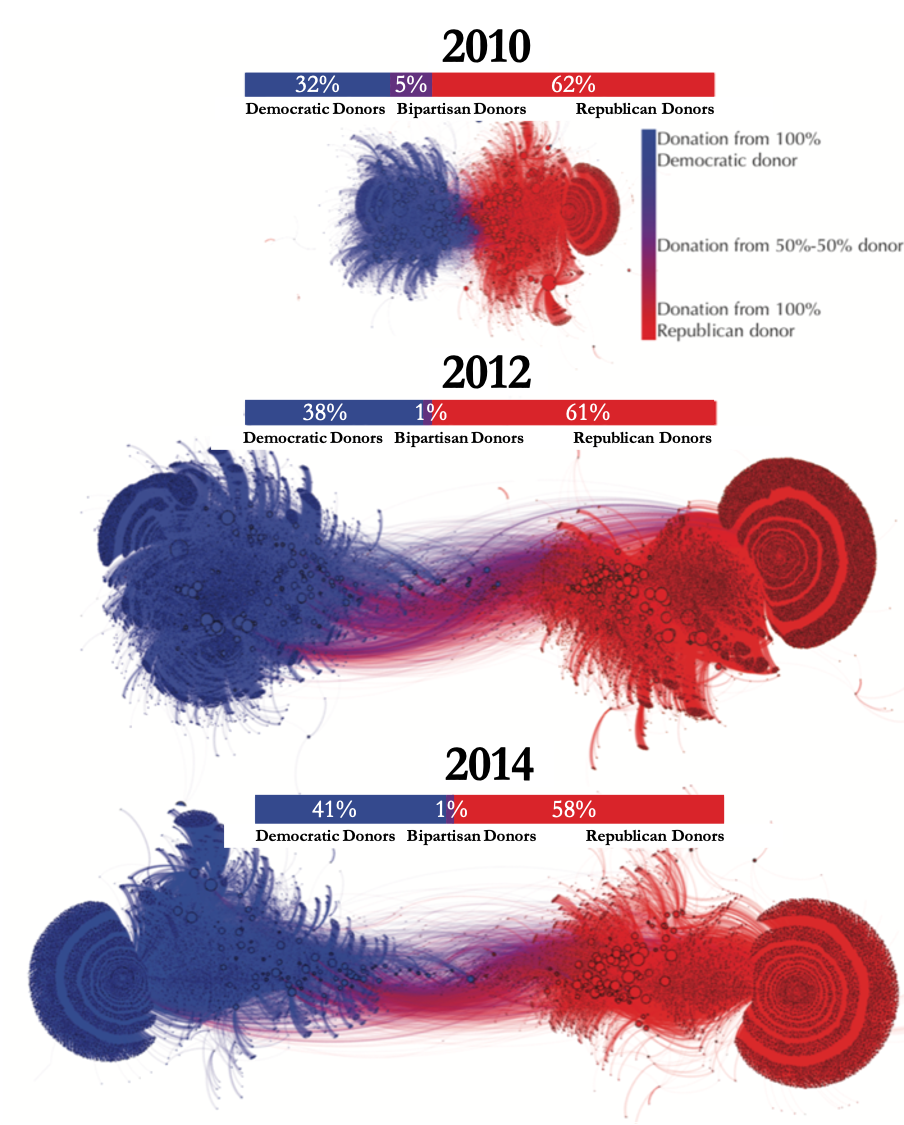
\includegraphics[width=0.73\linewidth]{../figures/fig1} 

}

\caption{Visual representation of Wisconsin donor networks in the 2010, 2012 and 2014 election cycle using the Yifan Hu layout algorithm. Each dot/ node is a donor or campaign and lines/ edges connecting them are donations. Nodes sized by in-degree (incoming donations. Nodes and edges are colored by the partisanship of the donor. Percentages on the bars represent the percent of donors in each party bin.}\label{fig:unnamed-chunk-11}
\end{figure}

\newpage

\hypertarget{figure-2}{%
\subsubsection{Figure 2}\label{figure-2}}

\begin{figure}
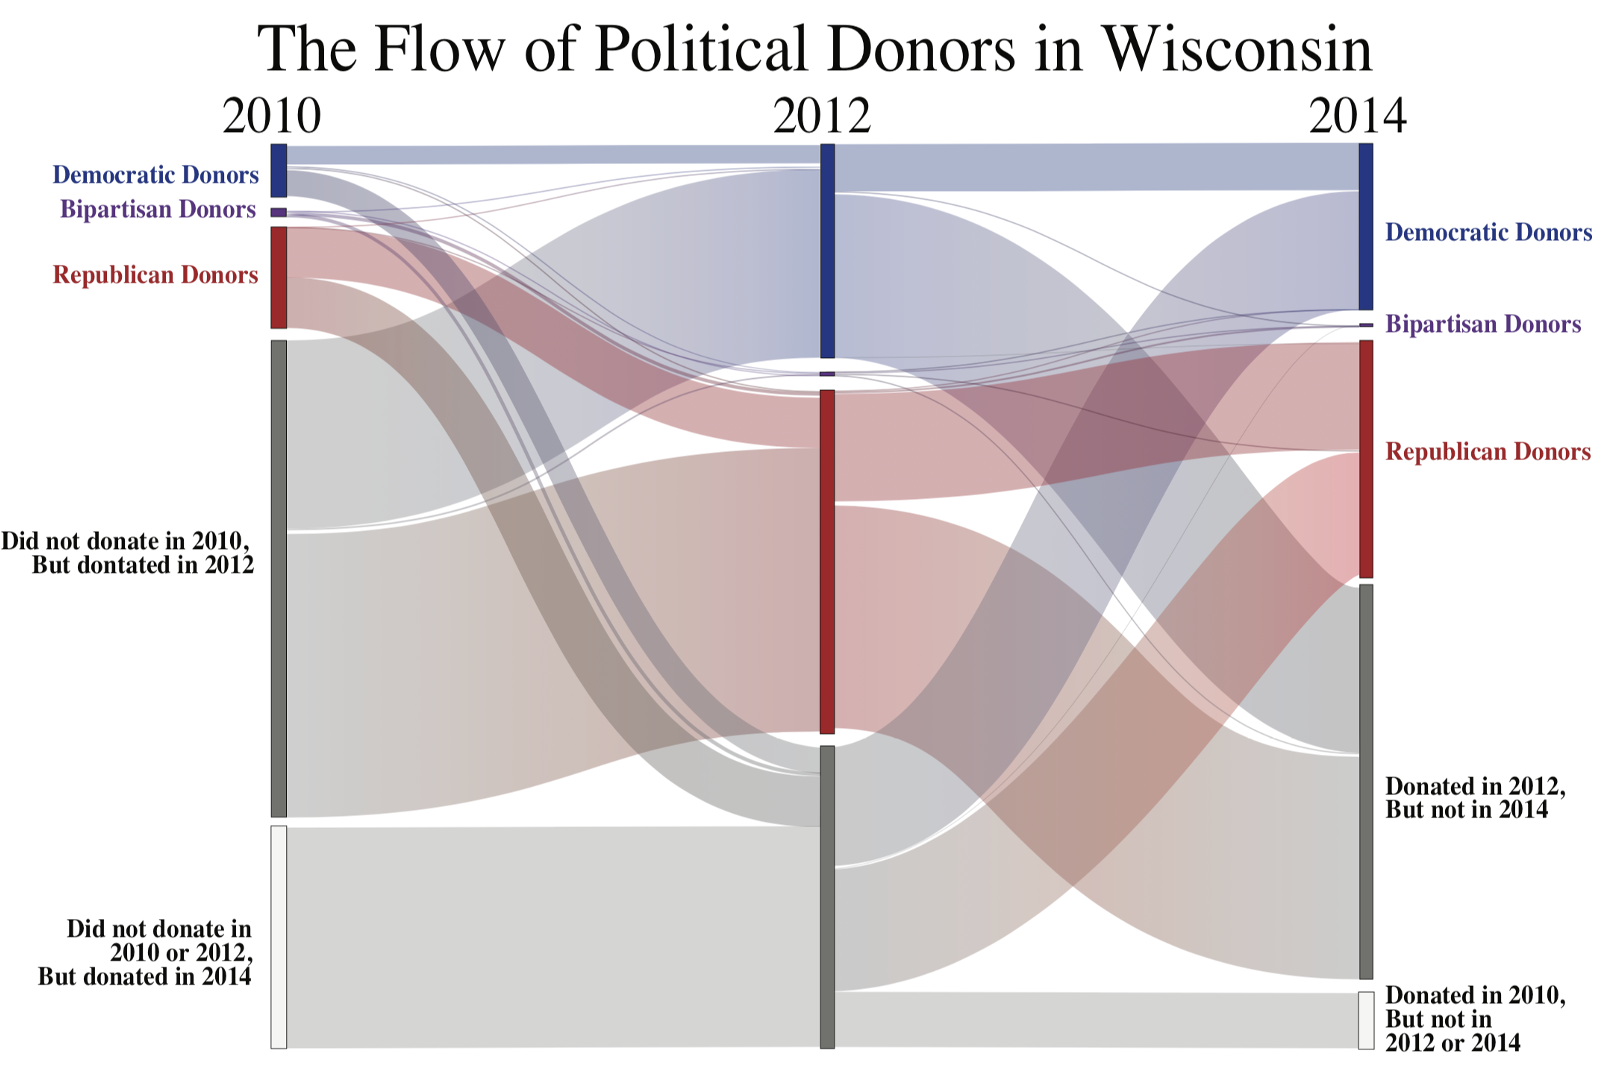
\includegraphics[width=1\linewidth]{../figures/fig2} \caption{Sankey diagram of the flow of political donors in 2010, 2012, and 2014 election cycles in Wisconsin. The vertical bars are proportional to the number of donors in each bin.}\label{fig:unnamed-chunk-12}
\end{figure}

\newpage

\hypertarget{figure-3}{%
\subsubsection{Figure 3}\label{figure-3}}

\begin{figure}
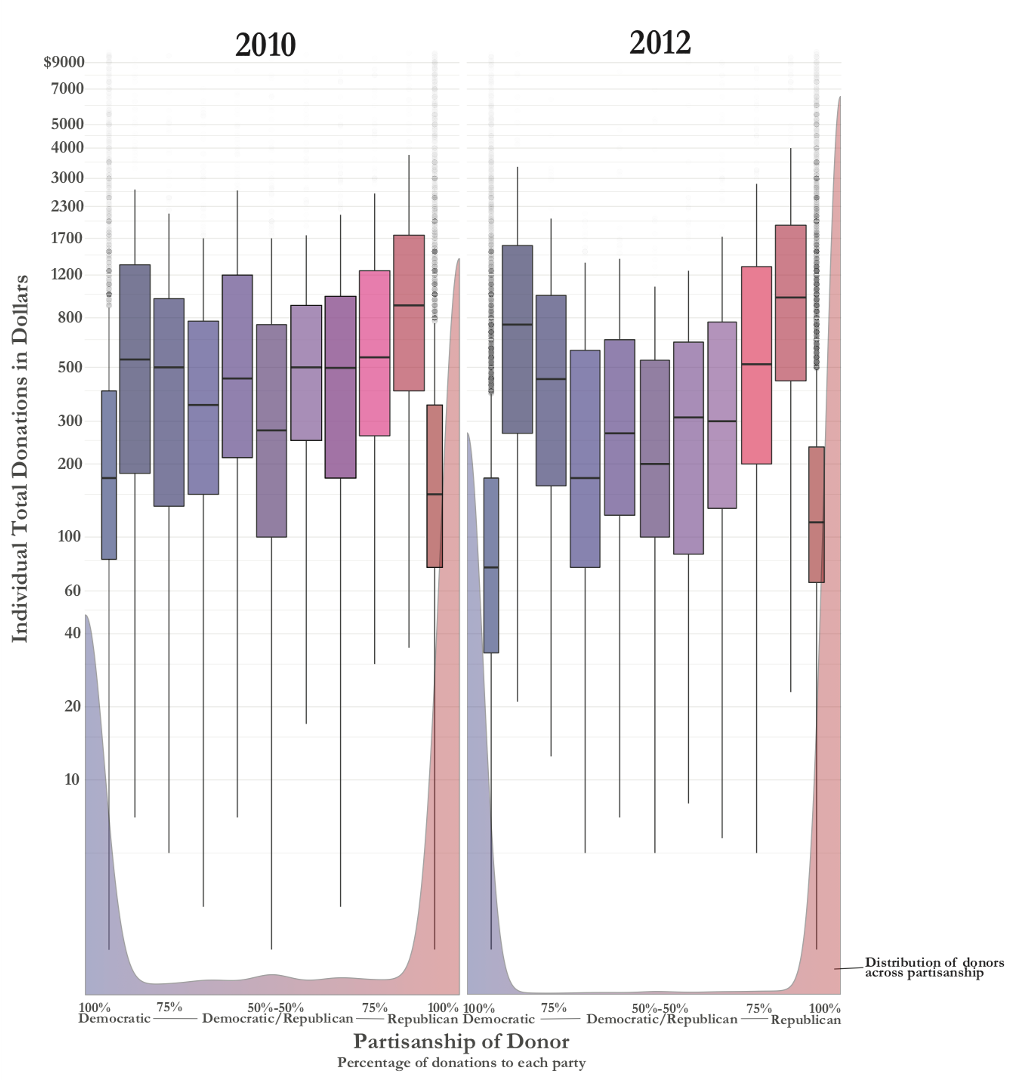
\includegraphics[width=0.9\linewidth]{../figures/fig4} \caption{This box and whisker plot is grouped by the partisanship of the donors in the 2010 and 2012 election cycles. Note that the y-axis is shown on a log10 scale for clarity. The partisan distribution is shown along the bottom of the x-axis.}\label{fig:unnamed-chunk-13}
\end{figure}

\newpage

\hypertarget{figure-4}{%
\subsubsection{Figure 4}\label{figure-4}}

\begin{figure}
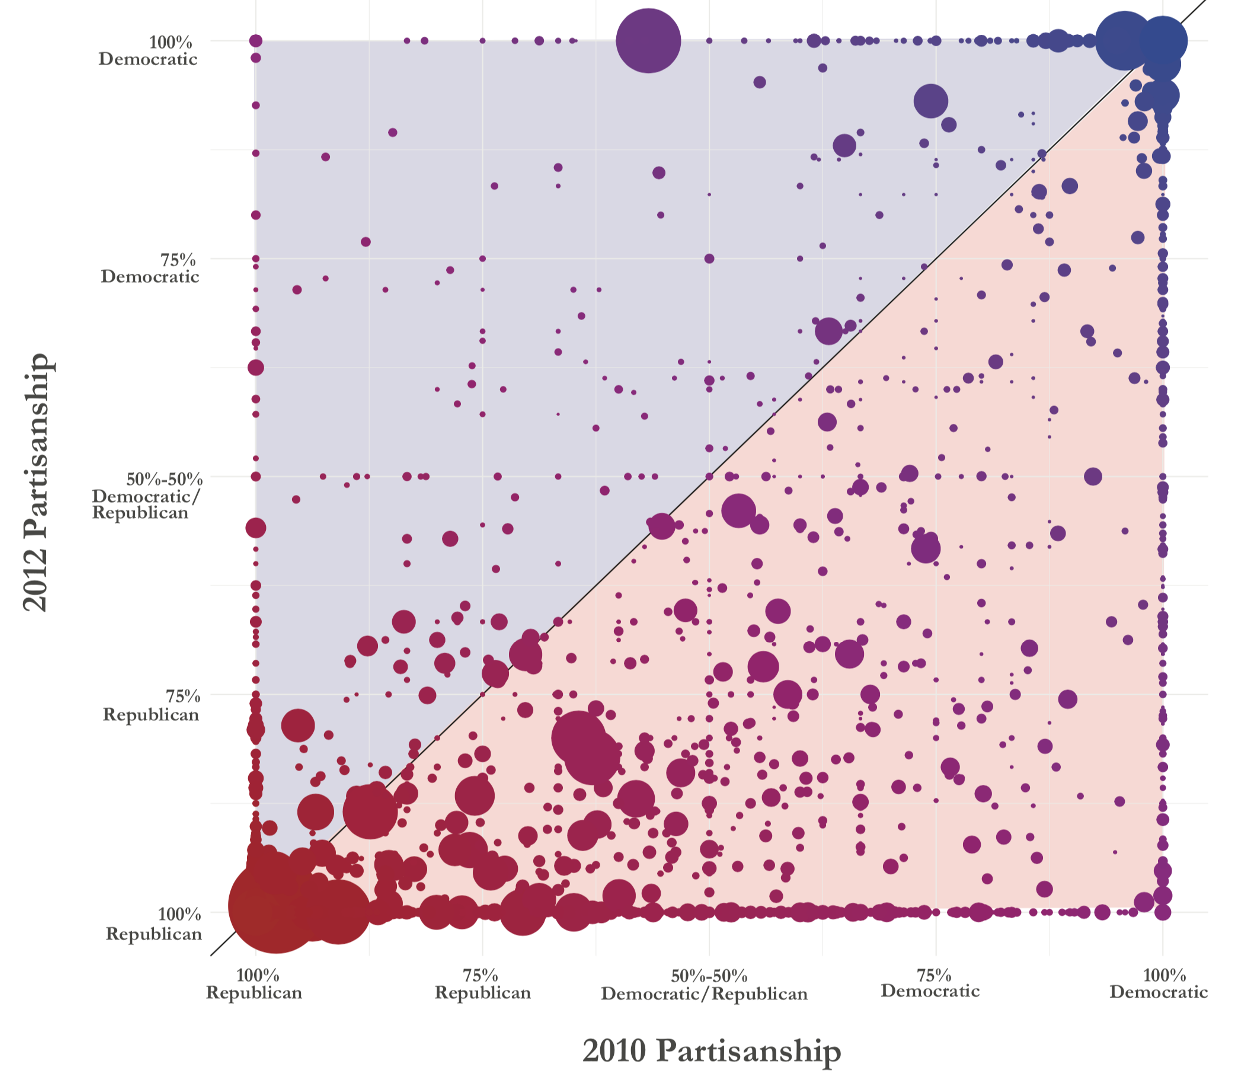
\includegraphics[width=1\linewidth]{../figures/fig3} \caption{Every dot is a donor who contributed in 2010 and 2012. The bigger the dot, the more money they contribted. The x-axis is their partisanship in the 2010 election cycle and the y-axis is their partisanship in the 2012 election cycle. If the donor is to the right of the center diagonal line, they became more Republican. If they are to the left of the line, they became more Democratic.}\label{fig:unnamed-chunk-14}
\end{figure}

\newpage

\hypertarget{figure-5}{%
\subsubsection{Figure 5}\label{figure-5}}

\begin{figure}
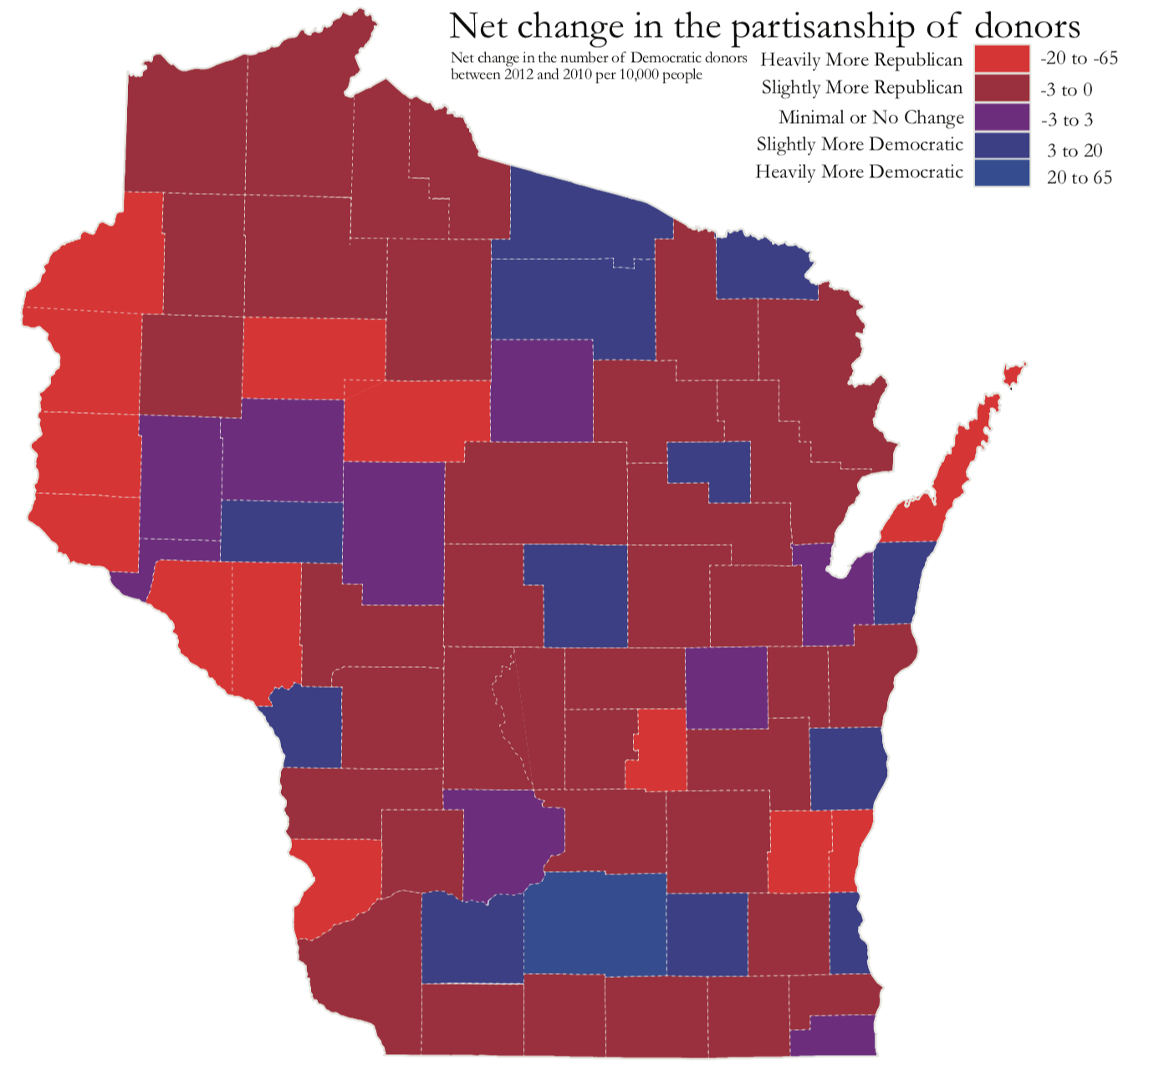
\includegraphics[width=0.9\linewidth]{../figures/fig5} \caption{This map shows the polarization of donor networks across Wisconsin's counties based on the net change of donors in each county per 10,000 residents. The red counties had a net increase in Republican donors, blue counties had a net increase for Democrats, and the purple counties had little or no change.}\label{fig:unnamed-chunk-15}
\end{figure}

\newpage

\hypertarget{references}{%
\section*{References}\label{references}}
\addcontentsline{toc}{section}{References}

\hypertarget{refs}{}
\leavevmode\hypertarget{ref-adalat2018}{}%
Adalat, Mohsin, Muaz A. Niazi, and Athanasios V. Vasilakos. 2018.
``Variations in Power of Opinion Leaders in Online Communication
Networks.'' \emph{Royal Society Open Science} 5 (10).

\leavevmode\hypertarget{ref-albert2020}{}%
Albert, Zachary, and Raymond La Raja. 2020. ``Small Dollar Donors and
the Evolving Democratic Party.'' \emph{American Political Science
Association Preprints}.

\leavevmode\hypertarget{ref-ansolabehere2003}{}%
Ansolabehere, Stephen, John M. de Figueiredo, and James M. Snyder Jr.
2003. ``Why Is There so Little Money in U.s. Politics.'' \emph{Journal
of Economic Perspectives} 17 (1): 105--30.

\leavevmode\hypertarget{ref-baker2019}{}%
Baker, Anne E. 2019. ``The Partisan and Policy Motivations of Political
Donors Seeking Surrogate Representation in House Elections.''
\emph{Political Behavior}, February.

\leavevmode\hypertarget{ref-barber2016a}{}%
Barber, Michael J. 2016. ``Ideological Donors, Contribution Limits, and
the Polarization of American Legislatures.'' \emph{The Journal of
Politics} 78 (1): 296--310.

\leavevmode\hypertarget{ref-barber2016b}{}%
Barber, Michael J., Daniel M. Butler, and Jessica Preece. 2016. ``Gender
Inequalities in Campaign Finance.'' \emph{Quarterly Journal of Political
Science} 1 (2): 219--48.

\leavevmode\hypertarget{ref-barber2016c}{}%
Barber, Michael J., Brandice Canes-Wrone, and Sharece Thrower. 2016.
``Ideologically Sophisticated Donors: Which Candidates Do Individual
Contributors Finance.'' \emph{American Journal of Political Science} 61
(2): 1057--72.

\leavevmode\hypertarget{ref-gephi}{}%
Bastian, Mathieu, Sebastien Heymann, and Mathieu Jacomy. 2009. ``Gephi:
An Open Source Software for Exploring and Manipulating Networks.''
\url{http://www.aaai.org/ocs/index.php/ICWSM/09/paper/view/154}.

\leavevmode\hypertarget{ref-blake2012}{}%
Blake, Aaron. 2012. ``Scott Walker Said Budget Strategy in Wisconsin Was
'Divide and Conquer'.'' \emph{The Washington Post}, May.

\leavevmode\hypertarget{ref-bode2018}{}%
Bode, Leticia, Stephanie Edgerly, Chris Wells, Itay Gabay, Charles
Franklin, Lew Friedland, and Dhavan V. Shah. 2018. ``Participation in
Contentious Politics: Rethinking the Roles of News, Social Media, and
Conversation Amid Divisiveness.'' \emph{Journal of Information
Technology \& Politics} 15 (3): 215--29.

\leavevmode\hypertarget{ref-bonica2017}{}%
Bonica, Adam. 2017. ``Professional Networks, Early Fundraising, and
Electoral Success.'' \emph{Election Law Journal: Rules, Politics, and
Policy} 16 (1): 153--71.

\leavevmode\hypertarget{ref-borsuk2017}{}%
Borsuk, Alan. 2017. ``New Poll Gives Vivid Look into Polarized Political
Perceptions.'' June 29, 2017.
\url{https://law.marquette.edu/poll/2017/06/29/new-poll-gives-vivid-look-into-polarized-political-perceptions/}.

\leavevmode\hypertarget{ref-bramlett2011}{}%
Bramlett, Brittany H., James G. Gimpel, and Frances E. Lee. 2011. ``The
Political Ecology of Opinion in Big-Donor Neighborhoods.''
\emph{Political Behavior} 33: 565--600.

\leavevmode\hypertarget{ref-infer}{}%
Bray, Andrew, Chester Ismay, Evgeni Chasnovski, Ben Baumer, Mine
Cetinkaya-Rundel, Simon Couch, Ted Laderas, et al. 2020. \emph{Infer:
Tidy Statistical Inference}.
\url{https://cran.r-project.org/web/packages/infer/index.html}.

\leavevmode\hypertarget{ref-bump2016}{}%
Bump, Philip. 2016. ``The Decline and Fall of Split-Ticket Voting,
Visualized.'' \emph{The Washington Post}, May.

\leavevmode\hypertarget{ref-cho2012}{}%
Cho, Wendy K. Tam, James G. Gimpel, and Iris S. Hui. 2012. ``Voter
Migration and the Geographic Sorting of the American Electorate.''
\emph{Annals of the Association of American Geographers} 103 (4):
856--70.

\leavevmode\hypertarget{ref-conover2011}{}%
Conover, Michael D., Jacob Ratkiewicz, M. Francisco, B. Gonçalves, F.
Menczer, and A. Flammini. 2011. ``Political Polarization on Twitter.''
In \emph{ICWSM}.

\leavevmode\hypertarget{ref-cramer2016}{}%
Cramer, K. J. 2016. \emph{The Politics of Resentment: Rural
Consciousness in Wisconsin and the Rise of Scott Walker}. Chicago
Studies in American Politics. University of Chicago Press.
\url{https://books.google.com/books?id=Rg2ZCwAAQBAJ}.

\leavevmode\hypertarget{ref-crowder-meyer2018}{}%
Crowder-Meyer, Melody, and Rosalyn Cooperman. 2018. ``Can't Buy Them
Love: How Party Culture Among Donors Contributes to the Party Gap in
Women's Representation.'' \emph{The Journal of Politics} 80 (4):
1211--24.

\leavevmode\hypertarget{ref-igraph}{}%
Csardi, Gabor, and Tamas Nepusz. 2006. ``The Igraph Software Package for
Complex Network Research.'' \emph{InterJournal} Complex Systems: 1695.
\url{http://igraph.org}.

\leavevmode\hypertarget{ref-desilver2016}{}%
Desilver, Drew. 2016. ``Split-Ticket District, Once Common, Are Now
Rare.'' \emph{Pew Research Center Fact Tank}, August.

\leavevmode\hypertarget{ref-francia2003}{}%
Francia, Peter L., John C. Green, Paul S. Herrnson, Lynda W. Powell, and
and Clyde Wilcox. 2003. \emph{The Financiers of Congressional
Elections}. New York, NY: Columbia University Press.

\leavevmode\hypertarget{ref-francia2005}{}%
Francia, Peter L., John C. Green, Paul S. Herrnson, Lynda W. Powell, and
Clyde Wilcox. 2005. ``Limousine Liberals and Corporate Conservatives:
The Financial Constituencies of the Democratic and Republican Parties.''
\emph{Social Science Quarterly} 86 (4): 761--78.

\leavevmode\hypertarget{ref-mlsp}{}%
Franklin, Charles. n.d. ``Marquette Law School Interactive Topline
Results.'' Marquette Law School Poll.
\url{https://lubarcenter.shinyapps.io/MLSPBook/}.

\leavevmode\hypertarget{ref-garcia2015}{}%
Garcia, David, Adiya Abisheva, Simon Schweighofer, Uwe Serdült, and
Frank Schweitzer. 2015. ``Ideological and Temporal Components of Network
Polarization in Online Political Participatory Media.'' \emph{Policy \&
Internet} 7 (1): 46--79.

\leavevmode\hypertarget{ref-gordon2007}{}%
Gordon, Sanford C., Catherine Hafer, and Dimitri Landa. 2007.
``Consumption or Investment? On Motivations for Political Giving.''
\emph{The Journal of Politics} 69 (4).

\leavevmode\hypertarget{ref-guerra2013}{}%
Guerra, P. H. Calais, Wagner Meira Jr., Clair Cardie, and R. Kleinberg.
2013. ``Party Polarization in Congress: A Network Science Approach.''
\emph{Proceedings of the 7th International Conference on Weblogs and
Social Media, ICWSM 2013}, January, 215--24.

\leavevmode\hypertarget{ref-harden2016}{}%
Harden, Jeffrey J., and Justin H. Kirkland. 2016. ``Do Campaign Donors
Influence Polarization? Evidence from Public Financing in the American
States.'' \emph{Legislative Studies Quarterly} 41 (1): 119--1542.

\leavevmode\hypertarget{ref-hemsley2015}{}%
Hemsley, Bronwyn, Stephen Dann, Stuart Palmer, Meredith Allan, and Susan
Balandin. 2015. ```We Definitely Need an Audience': Experiences of
Twitter, Twitter Networks and Tweet Content in Adults with Severe
Communication Disabilities Who Use Augmentative and Alternative
Communication (Aac).'' \emph{Disability and Rehabilitation} 37 (17):
1531--42. \url{https://doi.org/10.3109/09638288.2015.1045990}.

\leavevmode\hypertarget{ref-hill2017}{}%
Hill, Seth J., and Gregory A. Huber. 2017. ``Representativeness and
Motivations of the Contemporary Donorate: Results from Merged Survey and
Administrative Records.'' \emph{Political Behavior} 39 (March): 3--29.

\leavevmode\hypertarget{ref-yifanhu}{}%
Hu, Yifan. 2005. ``Efficient, High-Quality Force-Directed Graph
Drawing.'' \emph{Mathematica Journal} 10 (1): 37--71.

\leavevmode\hypertarget{ref-jacobson2012}{}%
Jacobson, Gary C. 2012. ``The Electoral Origins of Polarized Politics:
Evidence from the 2010 Cooperative Congressional Election Study.''
\emph{American Behavioral Scientist} 56 (12): 1612--30.

\leavevmode\hypertarget{ref-kaufman2012}{}%
Kaufman, Dan. 2012. ``How Did Wisconsin Become the Most Politically
Divisive Place in America?'' \emph{The New York Times Magazine}, May.

\leavevmode\hypertarget{ref-keena2019}{}%
Keena, Alex, and Misty Knight-Finley. 2019. ``Are Small Donors
Polarizing? A Longitudinal Study of the Senate.'' \emph{Election Law
Journal: Rules, Politics, and Policy} 18 (2): 132--44.

\leavevmode\hypertarget{ref-openrefine}{}%
Kelli, Ham. 2013. ``OpenReinfe (Version 2.5).'' \emph{Journal of the
Medical Library Association} 101 (3): 233--34.

\leavevmode\hypertarget{ref-khonsari2010}{}%
Khonsari, K. K., Z. A. Nayeri, A. Fathalian, and L. Fathalian. 2010.
``Social Network Analysis of Iran's Green Movement Opposition Groups
Using Twitter.'' In \emph{2010 International Conference on Advances in
Social Networks Analysis and Mining}, 414--15.

\leavevmode\hypertarget{ref-kinsella2015}{}%
Kinsella, Chad, Colleen McTague, and Kevin N. Raleigh. 2015. ``Unmasking
Geographic Polarization and Clustering: A Micro-Scalar Analysis of
Partisan Voting Behavior.'' \emph{Applied Geography} 62 (August):
404--19.

\leavevmode\hypertarget{ref-kitchens2016}{}%
Kitchens, Karin E., and Michele L. Swers. 2016. ``Why Aren't There More
Republican Women in Congress? Gender, Partisanship, and Fundraising
Support in the 2010 and 2012 Elections.'' \emph{Politics \& Gender} 12
(4): 648--76.

\leavevmode\hypertarget{ref-uwsc}{}%
Kniss, Chad J. 2010. ``UW Badger Poll™.'' UW Badger Poll. University of
Wisconsin-Madison, Madison, WI: University of Wisconsin Survey Center.
\url{https://web.archive.org/web/20140829043452/http://www.uwsc.wisc.edu/BP30PressRelease1_GovRace.pdf}.

\leavevmode\hypertarget{ref-laurison2016}{}%
Laurison, Daniel. 2016. ``Social Class and Political Engagement in the
United States.'' \emph{Sociology Compass} 10 (9): 684--97.

\leavevmode\hypertarget{ref-layton2011}{}%
Layton, Lyndsey. 2011. ``'Wisconsin 14' Group of Democratic Senators
Returns, Greeted by Thousands at Capitol.'' \emph{The Washington Post},
March.

\leavevmode\hypertarget{ref-lott2019}{}%
Lott, Maxim. 2019. ``Trump Campaign's Small-Dollar Donations Surge,
Marking Major Shift for Gop.'' \emph{Fox News}, August.

\leavevmode\hypertarget{ref-marley2019}{}%
Marley, Patrick, and Molly Beck. 2019. ``Divisive Politics Ruled
Wisconsin over the Last Decade.'' \emph{Milwaukee Journal Sentinel},
December.

\leavevmode\hypertarget{ref-mccarty2006}{}%
McCarty, Nolan, Keith T. Poole, and Howard Rosenthal. 2006.
\emph{Polarizaed America: The Dancedance of Ideology and Unequal
Riches}. Cambridge, Mass: MIT Press.

\leavevmode\hypertarget{ref-refinr}{}%
Muir, Chris. 2018. \emph{Refinr: Cluster and Merge Similar Values Within
a Character Vector}.
\url{https://cran.r-project.org/web/packages/refinr/index.html}.

\leavevmode\hypertarget{ref-newman2006}{}%
Newman, M. E. J. 2006. ``Modularity and Community Structure in
Networks.'' \emph{Proceedings of the National Academy of Sciences} 103
(23): 8577--82. \url{https://doi.org/10.1073/pnas.0601602103}.

\leavevmode\hypertarget{ref-oklobzija}{}%
Oklobdzija, Stan. 2016. ``Closing down and Cashing in: Extremism and
Political Fundraising.'' \emph{State Politics \& Policy Quarterly} 17
(2): 201--24.

\leavevmode\hypertarget{ref-pew2017}{}%
Pew Research Center. 2017. ``The Partisan Divide on Political Values
Grows Even Wider.'' online.

\leavevmode\hypertarget{ref-laraja2011}{}%
Raja, Raymond J. La, and David L. Wiltse. 2012. ``Don't Blame Donors for
Ideological Polarization of Political Parties: Ideological Change and
Stability Among Political Contributors, 1972-2008.'' \emph{American
Politics Research} 40 (3): 501--30.

\leavevmode\hypertarget{ref-r}{}%
R Core Team. 2013. \emph{R: A Language and Environment for Statistical
Computing}. Vienna, Austria: R Foundation for Statistical Computing.
\url{http://www.R-project.org/}.

\leavevmode\hypertarget{ref-rehman2020}{}%
Rehman, Ateeq Ur, Aimin Jiang, Abdul Rehman, Anand Paul, Sadia din, and
Muhammad Tariq Sadiq. 2020. ``Identification and Role of Opinion Leaders
in Information Diffusion for Online Discussion Network.'' \emph{Journal
of Ambient Intelligence and Humanized Computing}, January.

\leavevmode\hypertarget{ref-roscoe2005}{}%
Roscoe, Douglas D., and Shannon Jenkins. 2005. ``A Meta-Analysis of
Campaign Contributions' Impact on Roll Call Voting.'' \emph{Social
Science Quartlery} 86 (1): 52--68.

\leavevmode\hypertarget{ref-sewell2011}{}%
Sewell, Abby. 2011. ``Protesters Out in Force Nationwide to Oppose
Wisconsin's Anti-Union Bill.'' \emph{Los Angeles Times}, February.

\leavevmode\hypertarget{ref-shor2015}{}%
Shor, Boris. 2015. ``Polarization in American State Legislatures.'' In
\emph{American Gridlock: The Sources, Character, and Impact of Political
Polarization}, edited by James A. Thurber and AntoineEditors Yoshinaka,
203--21. Cambridge University Press.
\url{https://doi.org/10.1017/CBO9781316287002.011}.

\leavevmode\hypertarget{ref-skelley2018}{}%
Skelley, Geoffrey. 2018. ``Split-Ticket Voting Hit a New Low in 2018
Senate and Governor Race.'' \emph{FiveThirtyEight}, January.

\leavevmode\hypertarget{ref-stratmann1991}{}%
Stratmann, Thomas. 1991. ``What Do Campaign Contributions Buy?
Deciphering Causal Effects of Money and Votes.'' \emph{Southern Economic
Journal} 57 (3): 606--20.

\leavevmode\hypertarget{ref-thomsen2017}{}%
Thomsen, Danielle M., and Michele L. Swers. 2017. ``Which Women Can Run?
Gender, Partisanship, and Candidate Donor Networks.'' \emph{Political
Research Quarterly} 70 (2): 449--63.

\leavevmode\hypertarget{ref-torres-spelliscy2017}{}%
Torres-Spelliscy, Ciara. 2017. ``Time Suck: How the Fundraising
Treadmill Diminishes Effetive Governance.'' \emph{Seton Hall Legislative
Journal} 42 (December).

\leavevmode\hypertarget{ref-waugh2009}{}%
Waugh, Andrew Scott, Liuyi Pei, James H. Fowler, Peter J. Mucha, and
Mason Alexander Porter. n.d. ``Party Polarization in Congress: A Network
Science Approach.''

\leavevmode\hypertarget{ref-tidyverse}{}%
Wickham, Hadley, Mara Averick, Jennifer Bryan, Winston Chang, Lucy
D'Agostino McGowan, Romain François, Garrett Grolemund, et al. 2019.
``Welcome to the tidyverse.'' \emph{Journal of Open Source Software} 4
(43): 1686. \url{https://doi.org/10.21105/joss.01686}.

\leavevmode\hypertarget{ref-cfis}{}%
``Wisconsin Campaign Information System.'' n.d.
\url{https://cfis.wi.gov/\#}.

\leavevmode\hypertarget{ref-zhang2008}{}%
Zhang, Yan, A. J. Friend, Amanda L. Traud, Mason A. Porter, James H.
Fowler, and Peter J. Mucha. 2008. ``Community Sructure in Congressional
Cosponsorship Networks.'' \emph{Physica A: Statistical MEchanics and Its
Applications} 387 (1): 1705--12.





\newpage
\singlespacing 
\end{document}
